{下图给出了调度层次的示意图。从图中可以看出,一个作业从提交开始直到完成,往往要经历三级调度。}

{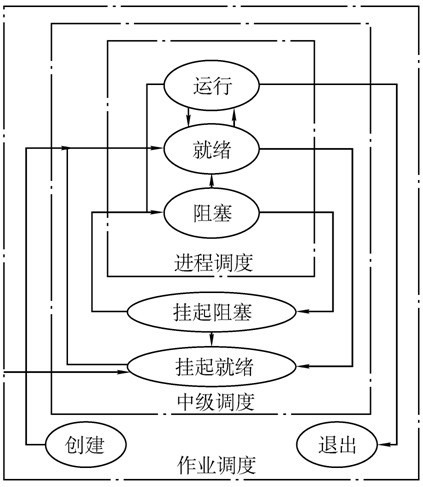
\includegraphics[width=3.33333in,height=3.83333in]{png-jpeg-pics/465B11B15425DACD970C7DB1B32AFF97.png}\\
}

\textbf{{1.高级调度(作业调度)}}

高级调度又称为宏观调度、作业调度或者长程调度,其{主要任务是按照一定的原则从外存上处于后备状态的作业中选择一个或者多个},给它们分配内存、输入输出设备等必要资源,并建立相应的进程,以使该作业具有获得竞争处理器的权利。

\textbf{{2.中级调度}}

中级调度又称为中程调度或者交换调度,其{主}{要任务是按照给定的原则和策略,将处于外存对换区中的具备运行条件的进程调入内存,或者将处于内存中的暂时不能运行的进程交换到外存对换区}\textbf{。}中级调度主要涉及内存管理与扩充(其实中级调度可以理解为在换页时将页面在外存与内存之间调度)。

\textbf{{3.低级调度(进程调度)}}

低级调度又称为微观调度、进程调度或者短程调度,其{主要任务是按照某种策略和方法从就绪队列中选取一个进程,将处理器分配给它}\textbf{。}进程调度的运行频率很高,一般隔几十毫秒要运行一次。后面将对此进行详细讲解。

\textbf{{4. 作业调度与进程调度区别}}

\textbf{1.~}{作业调度为进程被调用作准备,进程调度使进程被调用。换言之,}{作业调度的结果是为作业创建进程,而进程调度的结果是进程被执行}{。}

\textbf{2.~}作业调度次数少,进程调度频率高。

\textbf{3.~}有的系统可以不设置作业调度,但进程调度必须有。
